\documentclass[10pt,twocolumn]{article}

% use the oxycomps style file
\usepackage{oxycomps}

% usage: \fixme[comments describing issue]{text to be fixed}
% define \fixme as not doing anything special
\newcommand{\fixme}[2][]{#2}
% overwrite it so it shows up as red
\renewcommand{\fixme}[2][]{\textcolor{red}{#2}}
% overwrite it again so related text shows as footnotes
%\renewcommand{\fixme}[2][]{\textcolor{red}{#2\footnote{#1}}}

% read references.bib for the bibtex data
\bibliography{references}

% include metadata in the generated pdf file
\pdfinfo{
    /Title (NPL Tutorial)
    /Author (Ryann Hally)
}

% set the title and author information
\title{Tutorial: Fine-tuning a pretrained English to French machine translation model}
\author{Ryann Hally}
\affiliation{Occidental College}
\email{hally@oxy.edu}

\begin{document}

\maketitle
\section{Introduction}
For my comprehensive requirement I’m hoping to combine my interests in linguistics and computer science. This has led me to look into the field of natural language processing. While investigating current NLP areas of research, I read several articles on transfer learning for machine translation into low-resource languages. This refers when there aren't enough books, websites, social media posts, etc. in the language we want to translate into (the target language) to train a model from scratch. So, a model that's already been trained in translating into another language is fine-tuned for the target language. Researchers typically try to pick a language that is “linguistically similar” to the target language for pretraining. However, “linguistically similar” is never defined and could mean a number of things since there are several ways for languages to be related. Most selections seem to be based on assumed similarities from historical relationships. For example, using a model trained in translating into French to translate into Spanish because they are both romance languages. For my comprehensive requirement, I'd like to experiment with the languages the model is pretrained to translate into in order to better understand what linguistic similarities are most beneficial in transfer learning and how researchers can better pick language pairs.

To do this I will have to be able to select a pretrained machine translation model, find datasets in the target language I choose, fine-tune the model, and evaluate it's performance. I choose Hugging Face's machine translation tutorial, which covers these skills by walking readers through fine-tuning a model trained in English to French translation. 
A successful outcome for this would then be the model producing more accurate French translations after fine-tuning than it was before.


\section{Methods}

\subsection{The Dataset}
The dataset used for fine-tuning was the KDE4 dataset on Hugging Face, which is a collection of localized files for KDE apps in 92 different languages. The base language, or the language to be translated from, was English, and the target language was French. The dataset features 210,173 pairs of sentences.


\subsection{The Model}
The model used in this tutorial was a Marian model created by the Language Technology Research Group at the University of Helsinki. It had been pretrained in English to French translation on the Opus Dataset. 

Marian has a sequence-to-sequence architecture, meaning it is designed to both take in and output sequential data. Sequence-to-sequence models are encoder-decoder models. The encoder is what receives the input and builds a representation of it while the decoder is what generates the output sequence, giving it it's ability to input and output sequences. Marian is a transformer model, meaning it uses something called attention layers that direct the attention of the model to specific words. 

These features make the Marian model well equipped for machine translation. Machine translation models must take in and produce sequences of words. Additionally, the attention layers allow the model to take into account words that might influence the translation of a given word and ignore the ones that don't. 

The tokenizer, which converts the text into tokens that the model is able to take in as input, is based on the SentencePiece tokenizer. It is a subword tokenizer, meaning it leaves commonly used words as one token and splits infrequently used ones. SentencePiece is not language specific and can therefore be used for this tutorial.

\subsection{The tutorial}

\subsubsection{Data Preparation}
\hspace{\parindent}The first step is to prepare the data. For this tutorial, I had to divide the dataset into the English sentences and their French translations in order to create a validation set for fine-tuning. 

\subsubsection{Tokenization}
\hspace{\parindent}The second step is to tokenize the text. This first involved loading a compatible tokenizer. Then I created a preprocessing function to tell the tokenizer to process the text in the output language.


\subsubsection{Data Collation}
\hspace{\parindent}The third step of the tutorial is data collation. This involved loading a data collator to pad the inputs and labels so they are a compatible size for the model. 

\subsubsection{Evaluation}
\hspace{\parindent}The next step is evaluation. I installed sacreBLEU (see Metrics and Results) and evaluated the model so I could compare this score with the score it recieved after fine-tuning. I then had to create a function to process the outputs into text sacreBLEU could evaluate.

\subsubsection{Fine-Tuning}
\hspace{\parindent}The final step is to fine-tune the model. This involves defining the arguments of the training function and then training the model. The training speed used in the tutorial was not compatible with my setup on Google Colab and I had to deviate from the tutorial by lowering it. 

\section{Metrics and Results}
The goal of the tutorial was to teach readers how to fine-tune machine translation models by walking them through fine-tuning a Marian model trained in translating from English to French. A successful outcome would then be the model producing more accurate translations after fine-tuning than it was beforehand. This can be measured by evaluating the model before and after fine-tuning using a translation quality metric and comparing the scores. 

The translation quality metric used by the tutorial is the BLEU (BiLingual Evaluation Understudy). BLEU compares the n-grams of translated sequences produced by the model to the n-grams of sequences written by humans. It scores each sequence from 0 to 1 based on the number of matches. A model's final grade, or it's BLEU score, is the average of all the sequences it produced's scores. Figure 1 shows how the BLEU score is mathematically defined while Figure 2 shows the translation quality each BLEU score range indicates.

\begin{figure}
    \centering
    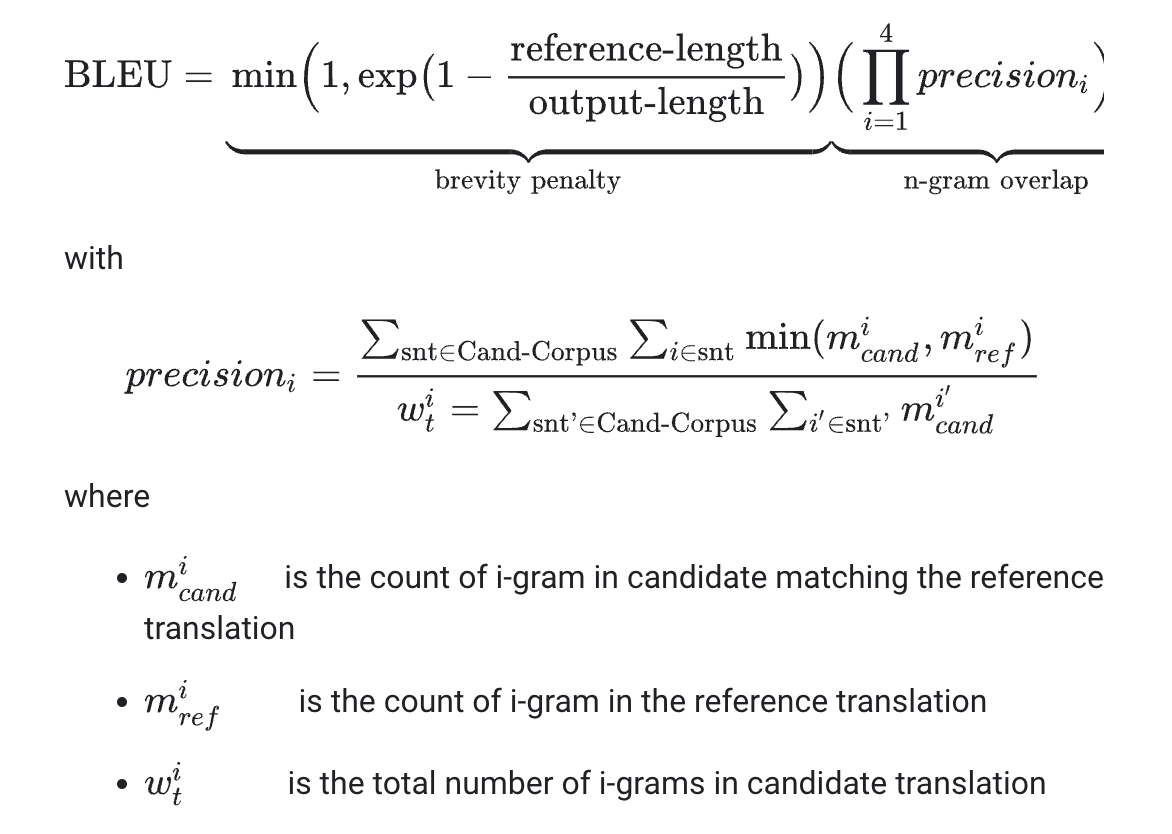
\includegraphics[width=.95\linewidth]{BLEUMathematicalDefinition.PNG}
    \caption{
        The mathematical definition of the BLEU score
    }
    \label{fig:first-page}
\end{figure}

\begin{figure}
    \centering
    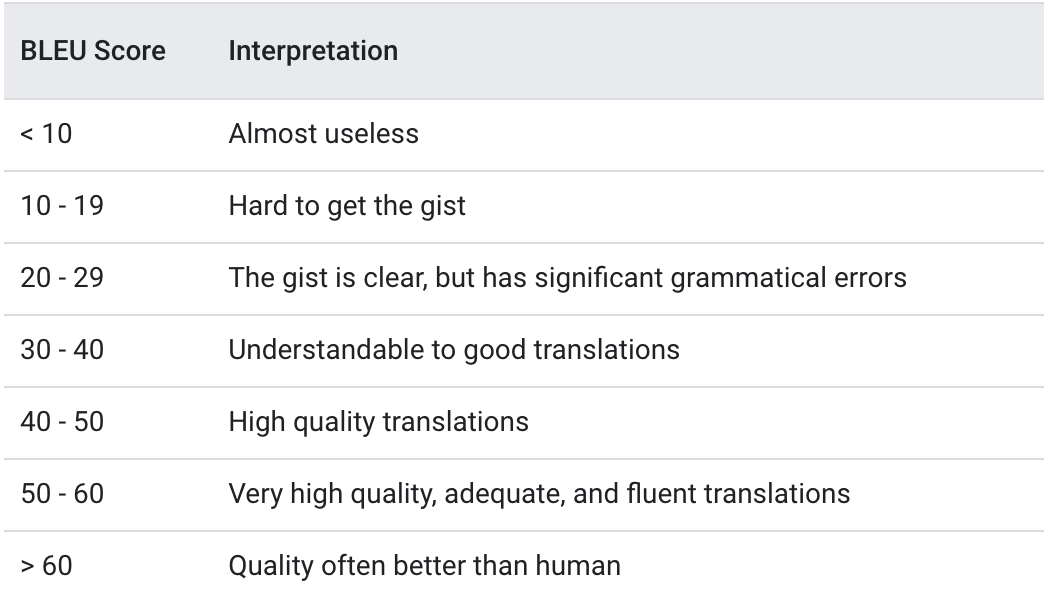
\includegraphics[width=.95\linewidth]{BLEUInterpretation.PNG}
    \caption{
        BLEU scores and indicated translation quality
    }
    \label{fig:first-page}
\end{figure}


The Marian model used in the tutorial received a BLEU score of 39.271 before fine-tuning, and a score of 52.894 after fine-tuning. This does indicate an improvement in translation accuracy and therefore a successful outcome for the tutorial. Additionally, as shown in Figure 2, this score indicates the model's translations prior to fine-tuning were ``understandable to good'' and were ``high quality'' after fine-tuning. 


\section{Reflection}
I find this topic interesting and I think there’s a lot to experiment with and discover. Overall, I feel good about this being my comprehensive requirement topic. The coding aspect of this tutorial was more straightforward than I expected and Hugging Face and libraries like Pytorch and TensorFlow make setting up and training the model very accessible. 
However, that's not to say the project will be easy. I think the difficulty will lie in understanding the different algorithms, architectures, components, and techniques well enough to make decisions about which one fits my project best. Even though all I did in this tutorial was fine-tune a pretrained model, I found the amount of choices I could make in regards to models, architectures, datasets, and tokenizers overwhelming. This is further complicated by the fact that not every tokenizer, for example, is compatible with every architecture. When I chose this tutorial, I was planning on following it exactly as intended once, and then replicating it with different models and languages. Despite the large amount of research I did in order to understand every part of the NLP pipeline, I did not feel like experimentation was possible as this point. However, I'm confident that I will be able to start deviating from tutorials once I get more familiar with the process and each component. 

One concern that I have is the environmental impact of the project. Even though I will be following the tutorial suggestion's to only use pretrained models to minimize carbon emissions from training, experimenting with different source languages means I'll have to repeatedly fine-tune the model I'm using. Hopefully this is something I can do more research on and find a way to fine-tune that is as environmentally friendly as possible.


\end{document}
